% Convert to .eps instructions:
% pdfcrop $2.pdf
% pdftops -f $1 -l $1 -eps "$2-crop.pdf"
% rm  "$2-crop.pdf"
% mv  "$2-crop.eps" $2.eps

\documentclass[tikz,border=5pt]{standalone}
% \documentclass[convert={outext=.eps, command=\unexpanded{pdftops -eps \infile}}]{standalone}

\newcommand{\VAR}{Success}

\input{\rootdir/includes/margins/zero_margins.tex}


\setlength{\voffset}{-1in}
\setlength{\hoffset}{-1in}
\usetikzlibrary{positioning}
\usetikzlibrary{shapes.geometric,calc}
% \usepackage{tikzexternal}
% \tikzexternalize

% Angle of incidence
\newcommand{\phiAngle}{35}   % 0 <  phi  < 45 : Controls left to right rotation
\newcommand{\thetaAngle}{30} % 0 < theta < 90 : Controls top to bottom rotation
\newcommand{\cosPhi}{cos(\phiAngle)}
\newcommand{\sinPhi}{sin(\phiAngle)}

% Equation font size
\newcommand{\EQS}{\Huge}

\newcommand{\cosTheta}{cos(\thetaAngle)}
\newcommand{\sinTheta}{sin(\thetaAngle)}

% Origin location
\newcommand{\OR}{0} % Origin

% Length of arrowed parts
\newcommand{\arrowL}{0.2}
\newcommand{\arrowLZ}{\arrowL/\cosTheta}
\newcommand{\coordL}{0.2}

% Lengths
\newcommand{\dx}{2}
\newcommand{\dy}{2}
\newcommand{\dz}{2}
\newcommand{\vol}{\dx*\dy*\dz}

% Projected lengths
\newcommand{\cosL}{\dz*\cosPhi*\sinPhi*\cosTheta}
\newcommand{\sinL}{\dz*\sinPhi*\cosPhi*\sinTheta}

% Coordinate location
\newcommand{\COx}{\dx+1.2} % Coordinate
\newcommand{\COy}{\dy-0.1} % Coordinate

% Cell center location
\newcommand{\CCx}{-{\cosL}/2+\OR+\dx/2}
\newcommand{\CCy}{-{\sinL}/2+\OR+\dy/2}

% Cell Face location
\newcommand{\Fx}{-{\cosL}/2+\OR,-{\sinL}/2+\dy/2+\OR}
\newcommand{\Fy}{-{\sinL}/2+\OR+\dy/2}

% Thickness of lines
\newcommand{\w}{1}
\newcommand{\wSquare}{\w}
\newcommand{\wCrissCross}{\w/2}
\newcommand{\wCoord}{\w}
\newcommand{\wArr}{4}
\newcommand{\s}{4.8} % New

% Arrow head type and direction
\newcommand{\arrL}{stealth-}
\newcommand{\arrR}{-stealth}
\newcommand{\arrLR}{-stealth-}

\begin{document}
\MOONSTITLE
\pagenumbering{gobble}
% For some reason, if -{\cosL} or {\sinL} is not the first term WITH a sign, compilation fails.
\noindent
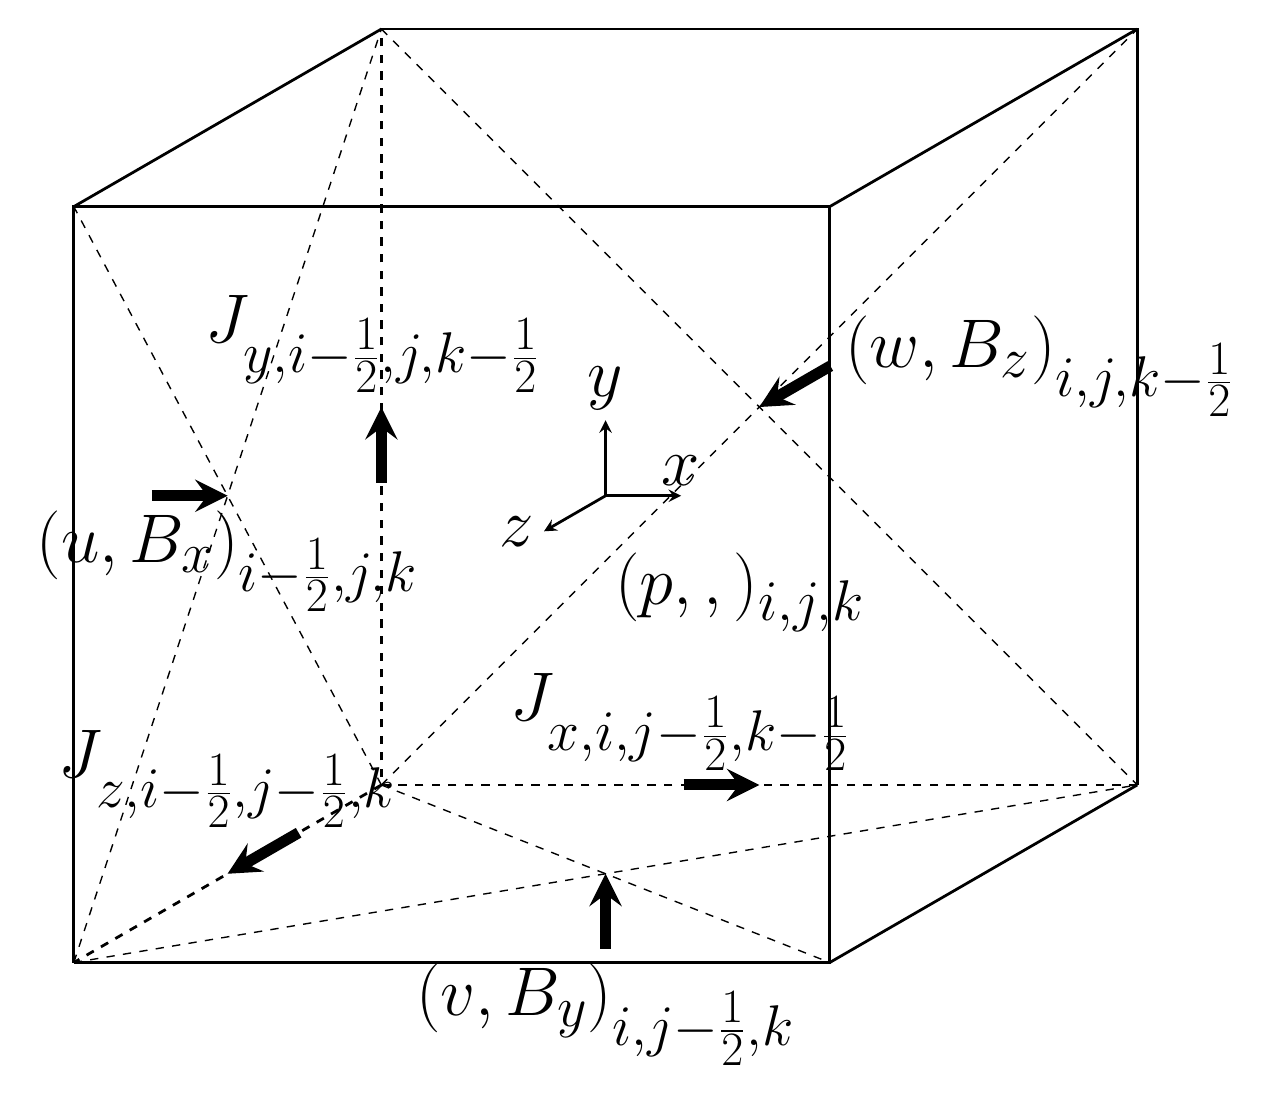
\begin{tikzpicture}[scale=\s]
\tikzstyle{every node}=[font=\LARGE]

% Cube lines:
	% Back face lines
	\draw[line width=\wSquare,dashed] (\OR+\dx,\OR) -- ++ (-\dx,0) -- ++ (0,\dy);
	\draw[line width=\wSquare]        (\OR+\dx,\OR) -- ++	(0,\dy) -- ++ (-\dx,0);
	% Front face lines
	\draw[line width=\wSquare] (-{\cosL}+\OR,-{\sinL}+\OR) -- ++ (\dx,0) -- ++ (0,\dy);
	\draw[line width=\wSquare] (-{\cosL}+\OR,-{\sinL}+\OR) -- ++ (0,\dy) -- ++ (\dx,0);
	% Diagonals lines
	\draw[line width=\wSquare,dashed] (\OR,\OR)         -- ++({-\cosL},{-\sinL});
	\draw[line width=\wSquare]        (\OR+\dx,\OR)     -- ++({-\cosL},{-\sinL});
	\draw[line width=\wSquare]        (\OR+\dx,\OR+\dy) -- ++({-\cosL},{-\sinL});
	\draw[line width=\wSquare]        (\OR,\OR+\dy)     -- ++({-\cosL},{-\sinL});

% Criss-cross lines (Sergey's request)
	\draw[line width=\wCrissCross,dashed] (\OR,\OR) -- ++(\dx,\dy);
	\draw[line width=\wCrissCross,dashed] (\OR,\OR) -- ++(-{\cosL}+\dx,-{\sinL});
	\draw[line width=\wCrissCross,dashed] (\OR,\OR) -- ++(-{\cosL},-{\sinL}+\dy);
	\draw[line width=\wCrissCross,dashed] (-{\cosL}+\OR,-{\sinL}+\OR) -- ++({\dx+\cosL},{\sinL});
	\draw[line width=\wCrissCross,dashed] (-{\cosL}+\OR,-{\sinL}+\OR) -- ++({\cosL},{\dy+\sinL});
	\draw[line width=\wCrissCross,dashed] (\OR,\OR+\dy) -- ++(\dx,-\dy);

% Edge fields:
	\draw[\arrR,anchor=east,line width=\wArr](\OR+\dx/2-\arrowL,\OR) -- ++(\arrowL,0)                                                               node[left=1,anchor=south]  {\EQS $J_{x,i,j-\frac{1}{2},k-\frac{1}{2}}$};
	\draw[\arrR,anchor=east,line width=\wArr](\OR,\OR+\dy/2-\arrowL) -- ++(0,\arrowL)                                                               node[left=.1,anchor=south]{\EQS $J_{y,i-\frac{1}{2},j,k-\frac{1}{2}}$};
	\draw[\arrR,anchor=east,line width=\wArr]({\OR-\cosL/2+\cosL*\arrowLZ},{\OR-\sinL/2+\sinL*\arrowLZ}) -- ++({-\cosL*\arrowLZ},{-\sinL*\arrowLZ}) node[above=.4,anchor=south]{\EQS $J_{z,i-\frac{1}{2},j-\frac{1}{2},k}$};

% Face fields:
	% \draw[line width=\wArr,\arrR] (\CCx-\dx/2-\arrowL,\CCy) -- ++(\arrowL,0)                     node[left=0.1,anchor=west] {\EQS $\ARRAY{l} u_{i-\frac{1}{2},j,k} \\ {B_x}_{i-\frac{1}{2},j,k} \EARRAY$};
	\draw[line width=\wArr,\arrR] (\CCx-\dx/2-\arrowL,\CCy) -- ++(\arrowL,0)                     node[anchor=north] {\EQS $(u,B_x)_{i-\frac{1}{2},j,k}$};
	\draw[line width=\wArr,\arrL] (\CCx,\CCy-\dy/2) -- ++(0,-\arrowL)                            node[anchor=north]         {\EQS $(v,B_y)_{i,j-\frac{1}{2},k}$};
	\draw[line width=\wArr,\arrL] (\OR+\dx/2,\OR+\dy/2) -- ++({\cosL*\arrowLZ},{\sinL*\arrowLZ}) node[anchor=west]          {\EQS $(w,B_z)_{i,j,k-\frac{1}{2}}$};

% Coordinate system (cell center)
	\draw[line width=\wCoord,\arrR]	(\CCx,\CCy) -- ++ (0,\coordL)                         node[anchor=south]{\EQS $y$};
	\draw[line width=\wCoord,\arrR]	(\CCx,\CCy) -- ++ (\coordL,0)                         node[anchor=south]{\EQS $x$};
	\draw[line width=\wCoord,\arrR]	(\CCx,\CCy) -- ++ ({-\cosL*\coordL},{-\sinL*\coordL}) node[anchor=east] {\EQS $z$};

% Cell center fields:
	% \draw [fill] (\CCx,\CCy) circle [radius=0.02];
	\draw (\CCx,\CCy) node[below=0.6,anchor=north west]{\EQS$ (p, \DEL \DOT \U, \DEL \DOT \B)_{i,j,k}$};

\end{tikzpicture}

\end{document}